\chapter{Computational Frameworks}
\label{frameworks}
\section{Overview}
\label{frameworks_overview}
\quad The problem of \textit{parallel software development} is multifaceted. To arrive at the final solution, a programmer has to work on multiple conceptual levels starting from problem decomposition and algorithm choice down to software architecture design, data structure choice, and finer-grained low-level loop transformations. If our loop parallelization assistant (see Chapter \ref{assistant}) aims at reducing the programmer's effort in the task of parallelizing a sequential program, the notion of computational frameworks and the library implementing it could be used in the process of developing a parallel application from the scratch. The solution we propose rids the programmer of the tasks of software architecture design, as well as algorithm and data structure choice by supplying a ready solution for parallelization of certain types of applications. The central motivating ground for the concept of computational frameworks is laid by the \textit{Data-Centric Parallelization (DCP)} problem, limitations of the related work, and the properties of the real world legacy codes.
\begin{center}
\textbf{\large \textit{Motivating ground for Computational Frameworks}}
\end{center}
\begin{description}[style=unboxed,leftmargin=0cm]
\itemsep0em
\item[\textit{The grand problem of Data-Centric Parallelization (DCP)}] Among all lower level implementation questions, the problem of successful data structure choice stands particularly prominent and important. Listings \ref{lst:frameworks_array} and \ref{lst:frameworks_list} illustrate how easily parallelization can be hampered. Both implementations solve an embarrassingly parallel problem of incrementing every sequence element by one. In the linear array based implementation compiler knows all element addresses statically and can generate parallel code. In the linked list based implementation compiler does not know element addresses in advance, since the latter will be resolved only dynamically and can generate only sequential code. Moreover, the data structure type is unknown to compiler. By parallelizable and non-parallelizable loops here we mean the loops that can and cannot be parallelized by the state-of-the-art compiler statically.\newline\null
\begin{minipage}[t]{0.5\linewidth}
\begin{lstlisting}[caption={\raggedright Parallelizable loop operating on what is clear to compiler a \textbf{linear array}.},label={lst:frameworks_array},language=C]
int a[1024];
for (int i=0; i<1024; i++) {
  a[i]=a[i]+1;
}
\end{lstlisting}
\end{minipage}
%
\begin{minipage}[t]{0.5\linewidth}
\begin{lstlisting}[caption={\raggedright Non-parallelizable loop operating on what programmer knows is a \textbf{linked-list}.},label={lst:frameworks_list},language=C]
struct Node* nptr;
for (p=nptr; p!=NULL; p=p->next) {
  p->value+=1;
}
\end{lstlisting}
\end{minipage}

If a programmer had a tool, that could automatically recognize the type and properties of data structures and automatically substitute them with a simpler, parallelizable and more suitable alternatives, that would make the parallelization process a lot easier. Unfortunately, as our state of the art overview discovered, the solution to the problem is not available yet. There are a lot of various techniques and methodologies with their specific limitations and problems.
\item[\textit{Data structure and algorithm inseparability}] An illustrative example in Listings \ref{lst:frameworks_array} and \ref{lst:frameworks_list} is obviously far below the complexity level of the real world code. The work with data structure can be spread all around the code base: allocation and initialization happen in one translation unit, update operations on the data structure are scattered between various functions in multiple other translation units. The exact way an operation works determines the properties (cyclicity, reachability, etc.) of a data structure and ultimately its type. It is crucial to understand how an algorithm actually calls data structure update operations. \textit{This all points to the inseparability of algorithms and data structures: understanding the type of the data structure might require understanding of the algorithm and vise versa; and the data structure substitution might lead to algorithm transformation.} Indeed, as our feasibility studies with the SPEC CPU2006 benchmark suite have shown (Section \ref{background_benchmarks_spec}) let alone automatic techniques, it might take some weeks for even an experienced human software engineer to understand what kind of data structures a benchmark uses and how to optimize it.
\item[\textit{Limitations of "The state of the art" work}] The discovery of higher level entities in programs is definitely not a novel idea. There are various \textit{static} and \textit{dynamic} techniques in the literature. \textit{Shape analysis} is one of the most well-known static techniques, which aims at understanding of various heap-allocated data structures and their properties (node reachability, cyclicity, disjointedness, etc.) at compile time \cite{Ghiya:1996:TDC:237721.237724}\cite{Sagiv:1999:PSA:292540.292552}\cite{Wilhelm:2000:SA:647476.760384}). \textit{Shape analysis techniques give a very rough and conservative approximation (a \textit{tree} instead of a \textit{linked list}), work with high error rates (\textit{DAG} instead of \textit{graph with cycles}) and are provably undecidable \cite{Muchnick:1998:ACD:286076}}. One of the more recent static techniques is based on pattern matching on the code intermediate representation (IR) level and aims at recognition of various computational idioms (such as reductions, stencils, sparse and dense linear algebra computations, etc.)\cite{Ginsbach:2017:DEG:3049832.3049862}\cite{Ginsbach:2018:CDS:3178372.3179515}\cite{Ginsbach:2018:AML:3296957.3173182}. Computational idioms are specified in a constraint-based domain specific programming language CAnDL. \textit{The technique allows for a rapid prototyping of new compiler optimizations based on pattern recognition and its substitution with an optimized versions of matched idioms, but it is limited for a relatively simple computational idioms and entities.} All static methods are limited in their program view to a single compilation unit. The challenge of data structure recognition requires a much broader view. Dynamic techniques come the closest to the solution of the DCP problem. There are numerous works available \cite{Haller:2016:SDS:2938006.2938029}\cite{Rupprecht:2017:DID:3155562.3155607}. These techniques are based on program instrumentation and construction of various dynamic memory allocation graphs. The idea is that these graphs along with their update operations can reflect the actual shape of the data structure. Probably, the most promising and the best performing of all is the work of a Data-structure Detection Tool (DDT) \cite{1669122}. The DDT tool can successfully recognise data structures in most of the standard libraries, such as STL, Apache (STDCXX), Borland (STLport), GLib, Trimaran achieving almost perfect recognition accuracy. Moreover, the technique has been able to recognise linked lists in Em3d and Bh Olden benchmarks. But, it is still far from solving the problem for an arbitrary real world code.
\item[\textit{The ongoing trend to higher abstraction levels}] For decades there has been an ongoing trend in the process of software engineering to move up in the levels of abstraction from bare hardware to higher level concepts closer to human reasoning and understanding. We have moved from assembly languages to languages like Fortran and C, followed by the development of object-oriented languages and a supplement of imperative programming languages with functional programming concepts. All these steps increase programmers productivity, improve program structuredness and modularity and move the process of software design closer to a human level. The trend of moving to higher abstraction levels is not only true for software engineering in general, but for parallel software engineering in particular. For example, standards like POSIX, OpenMP and MPI aim at abstracting a programmer from various hardware and operating system details and work on the level of platform agnostic parallel programming models. Parallel algorithmic skeletons \cite{mccool-patterns} (see Section \ref{background_skeletons}) move software parallelization process even higher and allow a programmer to specify a computation on the algorithmic level with various concepts like \textit{map}, \textit{stencil}, \textit{divide and conquer}, etc.
\end{description}
\begin{center}
\textbf{\large \textit{A higher level solution}}
\end{center}
\quad The task of separating data structures from algorithms for an arbitrary real world code is extremely challenging. Moreover, for some applications and benchmarks it does not seem meaningful either. For example, the suite of Olden benchmarks is much simpler, than SPEC CPU2006, but also exhibits the same inseparability problem. For many of Olden benchmarks the data structures and algorithms are blended, but the union they form can be framed into an elegant higher level entity, that can later be used to parallelize the benchmarks in a nice and structured way.\newline\null
\quad In this thesis we propose a novel notion of \textit{computational frameworks}, which exploit this possibility and help a programmer with a coarse-grained parallelization tasks, such as software design, algorithm and data structure choice on applications, where computations can be expressed with our computational frameworks. We describe the concept and the major frameworks in Section \ref{frameworks_main}. We provide a prototype C++ template library implementing the notion \cite{frameworks-repo} (see Section \ref{frameworks_library_design}). We prototyped the library on the suite of Olden benchmarks, which inspired and shaped the concept. The parallel library version consistently outperforms the sequential version hitting 5-6x speedups on the major benchmarks (see Section \ref{frameworks_performance}).
\subsection{Contributions of our Computational Frameworks}
\begin{itemize}[style=unboxed,leftmargin=0cm]
\itemsep0em
\renewcommand\labelitemi{$\vartriangleright$}
\renewcommand\labelitemii{$\bullet$}
\item We propose a novel notion of \textit{computational frameworks}, which are higher level entities that embody both data structures and algorithms; and
\item report on a prototype C++ template library \cite{frameworks-repo} implementing the notion in a modern, convenient, parallel and an easy to use way;
\item We express the computations of some Olden benchmarks in terms of our computational frameworks and rewrite their original sequential legacy C versions with the help of our library in a modern, better structured, portable and crucially parallel way (see Section \ref{frameworks_main});
\item We demonstrate the potential of the notion and the performance of the prototype library on the suite of Olden benchmarks (see Section \ref{frameworks_performance}), achieving consistent parallel speedups of 5-6x on the major benchmarks;
\item Finally, we propose an idea of alternative software parallelization approach based on our computational frameworks as a future work.
\end{itemize}
\section{Usage example}
\label{frameworks_usage_example}
\quad To get an initial feeling for what it is like to use our computational frameworks from a user perspective, let's consider a motivating example. A full discussion of the concept follows in Section \ref{frameworks_main}. Suppose we want to calculate a well-known functional programming concept of the \textit{right fold}, which also updates its elements with corresponding folded values, thus leaving some \textit{side effects}.\newline\null
\quad We can code that simple computation using the C++ Standard Template Library (STL). Listing \ref{lst:left_fold_list} shows the code implementing the task with an STL $list<> $ class template. First, we construct a list with 5 elements and initialize them to the value of 1. Then we loop through the list updating its elements and return the final right folded value. The task is small and the code is concise, but it is still possible to see its drawbacks. The code does not clearly separate concerns: list traversal, result computation and list transformation all happen in the same place and are mixed up together. For a better structuredness and comprehensibility it would make sense to put these different pieces of functionality into separate places. Alternatively, we could use STL's $std::accumulate()$ function template. The latter provides a programmer with a more concise and abstract interface, but does not allow any side effects. We would still need to write a separate chunk of code aimed at implementing an update of the list elements.\newline\null 
\quad Listing \ref{lst:left_fold_framework} shows an alternative implementation of the right fold using our \textbf{Fold} computational framework. The main computation here is expressed with a single line of code and a reader familiar with the concept of fold will comprehend the purpose of the code instantly. The fold defines the backbone of the computation, which is hidden from a user, while the definition of the custom part is left for a user to complete and is passed into a higher order functional style interface $Fold<Elem>::compute()$ as a function object $ComputeFunc$, which has been derived from a Fold-specific base class $Fold<Elem>::ComputeFunction<int>$. The latter is a template with the main computational result specified as a parameter. The base class frames the interface. Operator $Fold<Elem>::ComputeFunction<int>::operator()(Elem\&,int)$ takes an element of the Fold as an argument and combines it with the value folded so far in a user defined way. The user is supposed to pass the result further and has a freedom to update the element, thus leaving some side effects. The code in Listing \ref{lst:left_fold_framework} has a clear structure, but might feel a bit heavy for such a simple computation, but when a computational task is significant the advantages of the shown code design will become clear.

%\begin{minipage}[t]{\linewidth}
\begin{lstlisting}[caption={Right fold computation using standard STL list class template},label={lst:left_fold_list},language=C++]
#include <list>
using namespace std;

int main() {
    list<int> lst(5, 1);
    // lst = [ 1 <- 1 <- 1 <- 1 <- 1 ]
    
    int result = 0;
    for (auto it = lst.rbegin(); it != lst.rend(); it++) {
        *it += result;
        result = *it;
    }
    // lst = [ 5 <- 4 <- 3 <- 2 <- 1 ]
    // result = 5
    
    return 0;
}
\end{lstlisting}
%\end{minipage}

%\begin{minipage}[t]{\linewidth}
\begin{lstlisting}[caption={Right fold computation using our Fold computational framework},label={lst:left_fold_framework},language=C++]
#include "Fold.h"
using namespace abstract;

class Elem : public Fold<Elem>::Element {
    public:
        void grow() override { value = 1; }
        int value;
};

class ComputeFunc : public Fold<Elem>::ComputeFunction<int> {
    int operator()(Elem& elem, int fold) override {
        elem.value += fold;
        return elem.value;
    }
};

int main() {
    int fold_depth = 5;
    Fold<Elem> fold(fold_depth);
    // fold = [ 1 <- 1 <- 1 <- 1 <- 1 ]
    
    int result;
    ComputeFunc comp_func;
    result = fold.template compute<int>(comp_func);
    // fold = [ 5 <- 4 <- 3 <- 2 <- 1 ]
    // result = 5
    
    return 0;
}
\end{lstlisting}
%\end{minipage}

\section{Computational Frameworks}
\label{frameworks_main}
\quad In this section we describe the general concept of \textbf{computational framework} along with all frameworks we propose and implement in the prototype library. As our frameworks have been inspired by computations found in the Olden benchmark suite, it would be helpful to review the Section \ref{background_benchmarks_olden} describing the key benchmarks.
\subsection{The concept}
\label{frameworks_concept}
\quad As we have already mentioned the concept of \textit{computational framework} has been inspired by the current problems in the software parallelization field along with computational patterns we have observed in the suite of Olden benchmarks. Very often programs are written with sub optimal from the point of software parallelization data structures. It might be hard to substitute them with parallelizable alternatives as the former might be closely entangled with algorithms the program is based on. Hence:
\begin{itemize}[style=unboxed,leftmargin=0cm]
\itemsep0em
\renewcommand\labelitemi{$\vartriangleright$}
\renewcommand\labelitemii{$\bullet$}
\item Computational frameworks grow on the problem of data structure and algorithm inseparability;
\end{itemize}
\quad We might keep the two together, but still tackle the problem at a higher level. We call the higher level entity we operate with a computational framework. Computational emphasizes the algorithmic component, while framework hints towards the underlying data structure. 
\begin{itemize}[style=unboxed,leftmargin=0cm]
\itemsep0em
\renewcommand\labelitemi{$\vartriangleright$}
\renewcommand\labelitemii{$\bullet$}
\item Computational frameworks combine algorithms and data structures to form a higher level entity;
\end{itemize}
\quad Moreover, there are some specific problems, that could be tackled more effectively with specialized constructs. Imagine some task of scientific simulation. The scientific computation might be abundant with various higher level algorithmic constructs like maps, reductions, folds, stencils, etc. These concepts are characteristic of functional programming. The latter often forbids any mutable states. At the same time simulations often keep a significant state being updated and accumulated with every step. The presence of state is characteristic to an imperative programming. Here one can see a contradiction and hence the gap to fill: \begin{itemize}[style=unboxed,leftmargin=0cm]
\itemsep0em
\renewcommand\labelitemi{$\vartriangleright$}
\renewcommand\labelitemii{$\bullet$}
\item Computational frameworks fill the gap between imperative and functional programming paradigms;
\end{itemize}
\quad With all the things said above it is human programmers, who are going to use the concept in the end. Hence, it must be human friendly and convenient. At the same time the code must be modern and effective. We designed an object-oriented library with a functional style interface consisting of higher order functions. While the algorithmic component of the given framework is immutable there is a custom user defined functionality to apply to the framework. That functionality comes as a function object through the framework's interface in accordance with a command and template method (see Section \ref{background_design}) software design patterns. 
\begin{itemize}[style=unboxed,leftmargin=0cm]
\itemsep0em
\renewcommand\labelitemi{$\vartriangleright$}
\renewcommand\labelitemii{$\bullet$}
\item Computational frameworks provide a modern and convenient interface with elements of both functional, as well as object-oriented programming; and
\item Computational frameworks embody the best ideas of various software design patterns. 
\end{itemize}
\quad When the software architecture has been designed, the exact efficient algorithm has been chosen along with all the most optimal and suitable data structures supporting its operation, a programmer can move onto the task of software parallelization. Here:  
\begin{itemize}[style=unboxed,leftmargin=0cm]
\itemsep0em
\renewcommand\labelitemi{$\vartriangleright$}
\renewcommand\labelitemii{$\bullet$}
\item Computational frameworks implement an effective and portable parallelization under the hood.
\end{itemize}
\quad To conclude:
\begin{itemize}[style=unboxed,leftmargin=0cm]
\itemsep0em
\renewcommand\labelitemi{$\vartriangleright$}
\renewcommand\labelitemii{$\bullet$}
\item Computational frameworks improve program \textbf{structuredness}, \textbf{modularity}, \textbf{separation of concerns} and hide possible \textbf{program parallelization} behind the \textbf{modern and convenient} user interface. 
\end{itemize}
\subsection{Fractal}
\label{frameworks_fractal}
\quad The \textbf{Fractal} computational framework is the key framework in our work. It has been inspired by the theoretical work on tree reductions \cite{tree-reductions-paper} and 3 Olden benchmarks (\textit{health}, \textit{treeadd} and \textit{perimeter}) with a very similar computational pattern. Although, the work on tree reductions has laid the theoretical foundation, but it did not provide a practical implementation. While there are numerous computations, processes and examples, which can be framed into the fractal, for the simplest and the most illustrative example let's consider an n-ary tree data structure being processed as follows.\newline\null
\quad \textbf{Fractal's growth.} First, we grow the tree from the root down to its leaves. A node takes a seed to grow, grows and spawns the next set of seeds for all its children nodes. The latter continue the process of growth. In the most general case the growth can happen asymmetrically, i.e it can stop on some paths down the tree, when some user specified condition is met for some nodes. In other words, the tree becomes incomplete with some leaves growing deeper than others and some nodes not having some children. We saw that pattern in the \textit{perimeter} benchmark (see Section \ref{background_benchmarks_olden}), when squares fell completely outside or inside the ring, they stopped to split further. Benchmarks \textit{health} and \textit{treeadd} grow complete trees and do not specify any stop conditions. While the algorithmic pattern of growth is fixed, the node's growth itself along with the node's data are custom and user defined parts. The same is true of the type of seeds and seed spawning procedures. Moreover, the growth of the tree along its various branches happens independently and can be parallelized.\newline\null
\quad \textbf{Fractal's processing.} When the tree is grown, we can start to process it. On that stage we go in the opposite direction from the bottom up by starting to process the leaves of the tree first. For every node we do some custom computation along with updating its custom data and pass the computation's result up to its parent. Before we process any node we need to process all its children first. The processing of different children happens independently and can safely be parallelized. When the tree has been processed we obtain the final result from its root along with all the side effects left in the nodes of the tree. The user defines these side effects per node in the custom processing function along with defining the exact computation from children up to the parent. We can repeat the process numerous times. This is the way some simulations work. The side effects are going to accumulate and make the nodes heavier.
\begin{figure}[!htb]
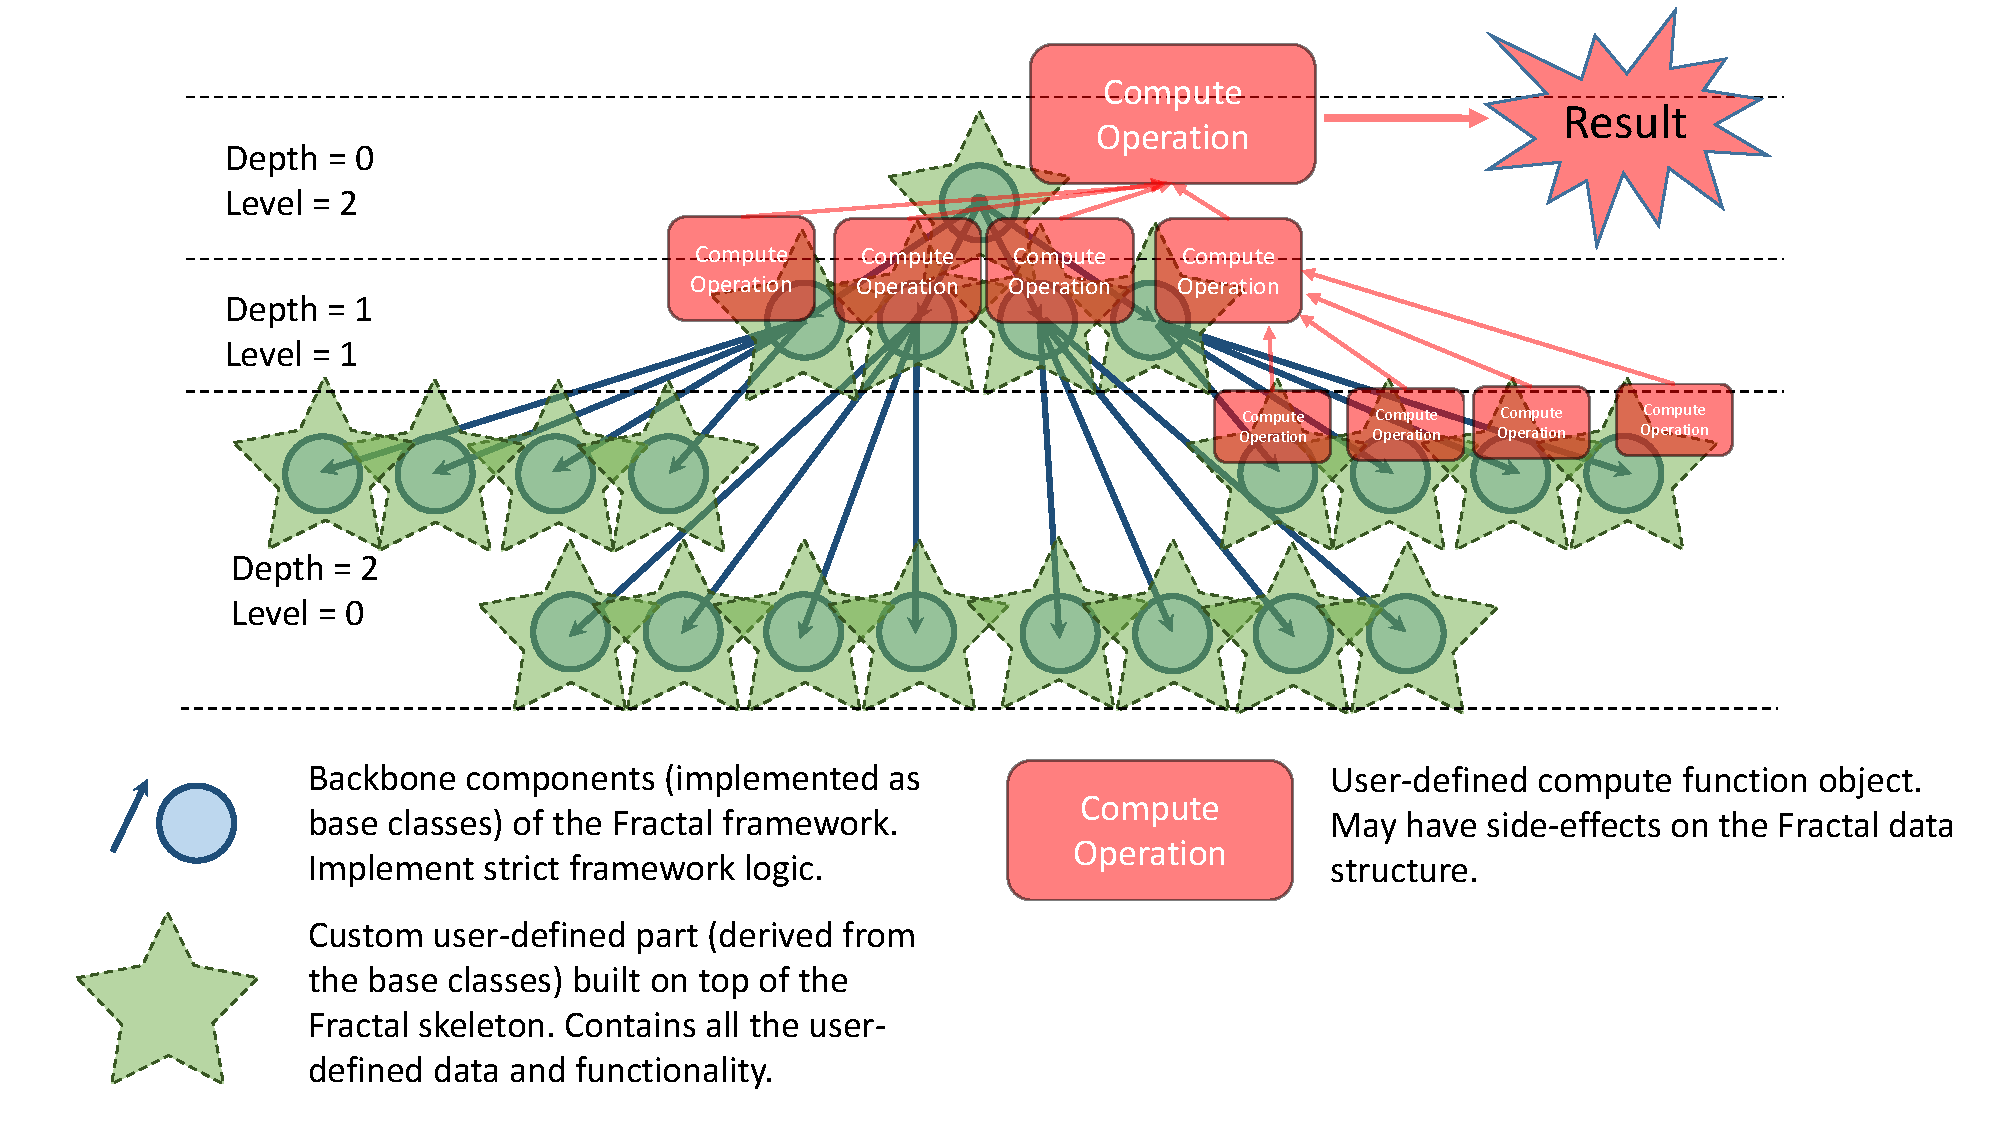
\includegraphics[width=1.0\textwidth]{images/Fractal.pdf}
\caption{Our object-oriented design of the Fractal computational framework.}
\label{fig:fractal_scheme}
\end{figure}
Figure \ref{fig:fractal_scheme} illustrates the pattern described above, as well as proposes an object-oriented design of the fractal concept. The backbone components (circles and arrows) of the tree are immutable and keep the main computational and growth patterns. These components can be implemented as base classes. Along with the backbone logic implementation these base classes provide a customizable interface to be overriden by derived classes (stars). Derived classes specify custom data contained in the tree nodes along with the exact growth and processing procedures, which can touch and alter the data. Given the fixed custom data in the tree nodes, computations operating on the data may still vary. We customize computations as function objects (red rectangles) being passed into higher order functional interfaces of the fractal. In other words, our fractal provides functional style interfaces above its object-oriented structure with the main backbone logic hidden under the hood. The backbone logic can be implemented sequentially or be parallelized in a multiple ways. In all its generality the fractal is a pattern, which can be characterized with self-similarity, repeatedness, structuredness, inherent parallelizability and the exact numeric values such as its depth and arity.
\subsection{Fold}
\label{frameworks_fold}
\quad The \textbf{Fold} computational framework has been inspired by the computation done in the \textit{power} benchmark (see Section \ref{background_benchmarks_olden}). The fold is not a new concept and has found a wide application in many functional languages. The C++ language provides \textit{std::accumulate()} function template as a component of its Standard Template Library (STL), which performs a functional fold over a given data structure, but contrary to our computational framework it does not allow any side-effects and modifications to the elements of the data structure must be coded separately. Our C++ \textit{Fold} class template provides an alternative interface to a user with an extensible customization space and clear separation of concerns.\newline\null
\begin{figure}[ht]
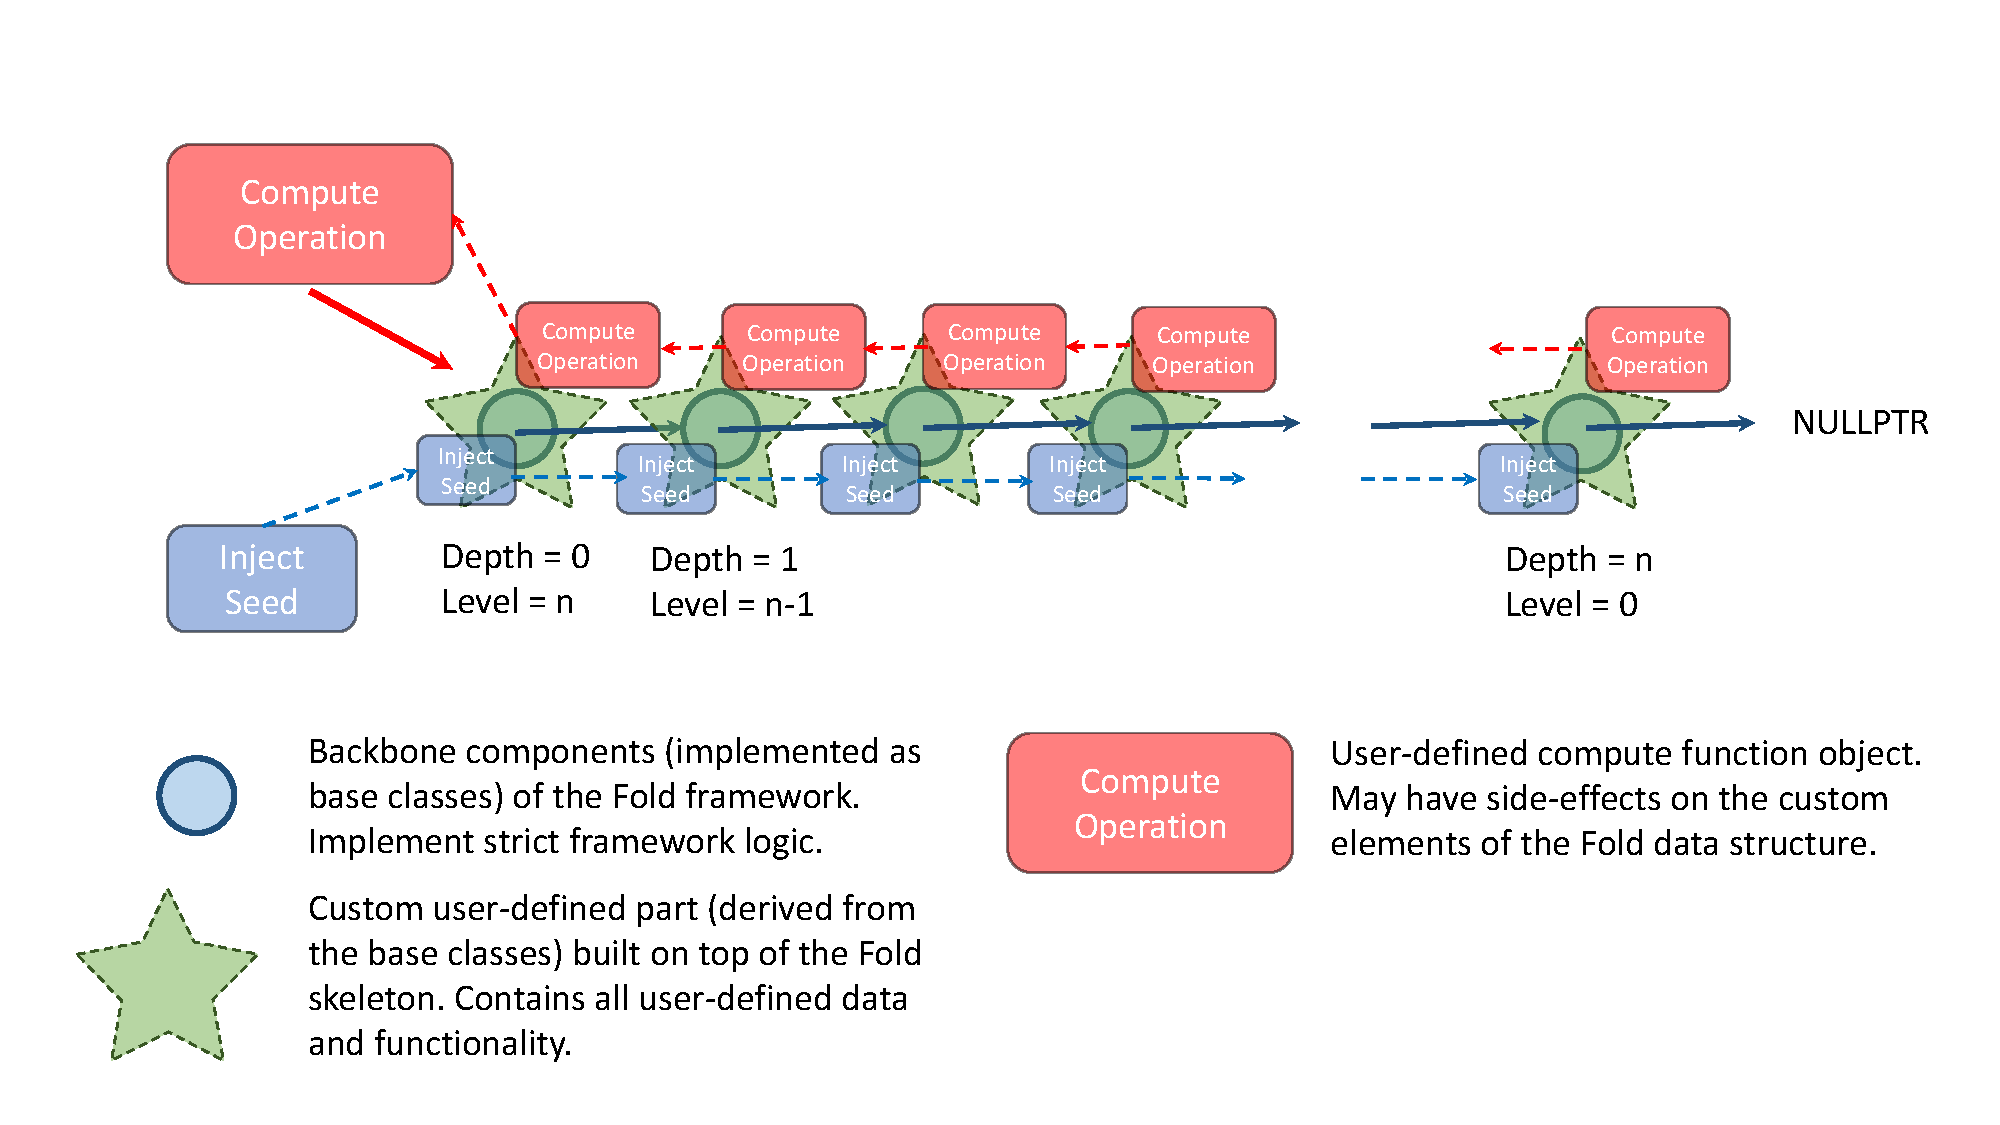
\includegraphics[width=1.0\textwidth]{images/Fold.pdf}
\caption{An object-oriented design of the Fold computational framework.}
\label{fig:fold}
\end{figure}\newline\null
\quad Figure \ref{fig:fold} illustrates the framework. One can think of a Fold as a set of elements arranged into a linked-list. We grow the list to the specified depth given a seed value. Then we may inject some data into the head of the list and propagate the data along with its custom changes to the last element at the tail of the list. All propagation modifications are user-defined. The injection of the data might happen as needed (before every fold iteration for example). Once every element of the list is ready with its injected data planted, the computation starts at the tail element and passes computed values back to previous elements of the chain. The computation may leave some side effects on the elements of the fold, which can accumulate with fold repetitions. The pattern is not parallelizable, but defines a strict order and helps to structure the code to separate various concerns. The object-oriented design of the fold framework is coherent to that of the fractal. Base classes form the skeleton logic and define the interface. All customization happens through overriding inherited base class interface methods withing definitions of derived classes. Custom compute operation is a function object going into functional interfaces of higher order \textit{Fold} class methods.
\subsection{Reduce}
\label{frameworks_reduce}
\quad Strictly speaking, \textbf{Reduce} is not a computational framework, but an algorithmic skeleton (see Section \ref{background_frameworks_vs_skeletons}). Although it is implemented with exactly the same design and interface, what illustrates compatibility between the two closely related concepts. The difference between our framework and \textit{std::reduce()} from C++ Standard Template Library (STL) is the possibility of having side effects and an alternative user customization interface. All general remarks made regarding \textbf{Fold} and \textbf{Fractal} frameworks also apply to the \textbf{Reduce} framework, although the specific details might differ. For example, the reduce framework takes a function object with two overloaded and virtual \textit{operator()} methods. One specifies how to reduce the value from a single element (possibly changing the element in the process) and the other defines the way of combining all the reduced values into the final return value. Our framework implements sequential as well as parallel \textbf{Reduce} versions.
\begin{figure}[ht]
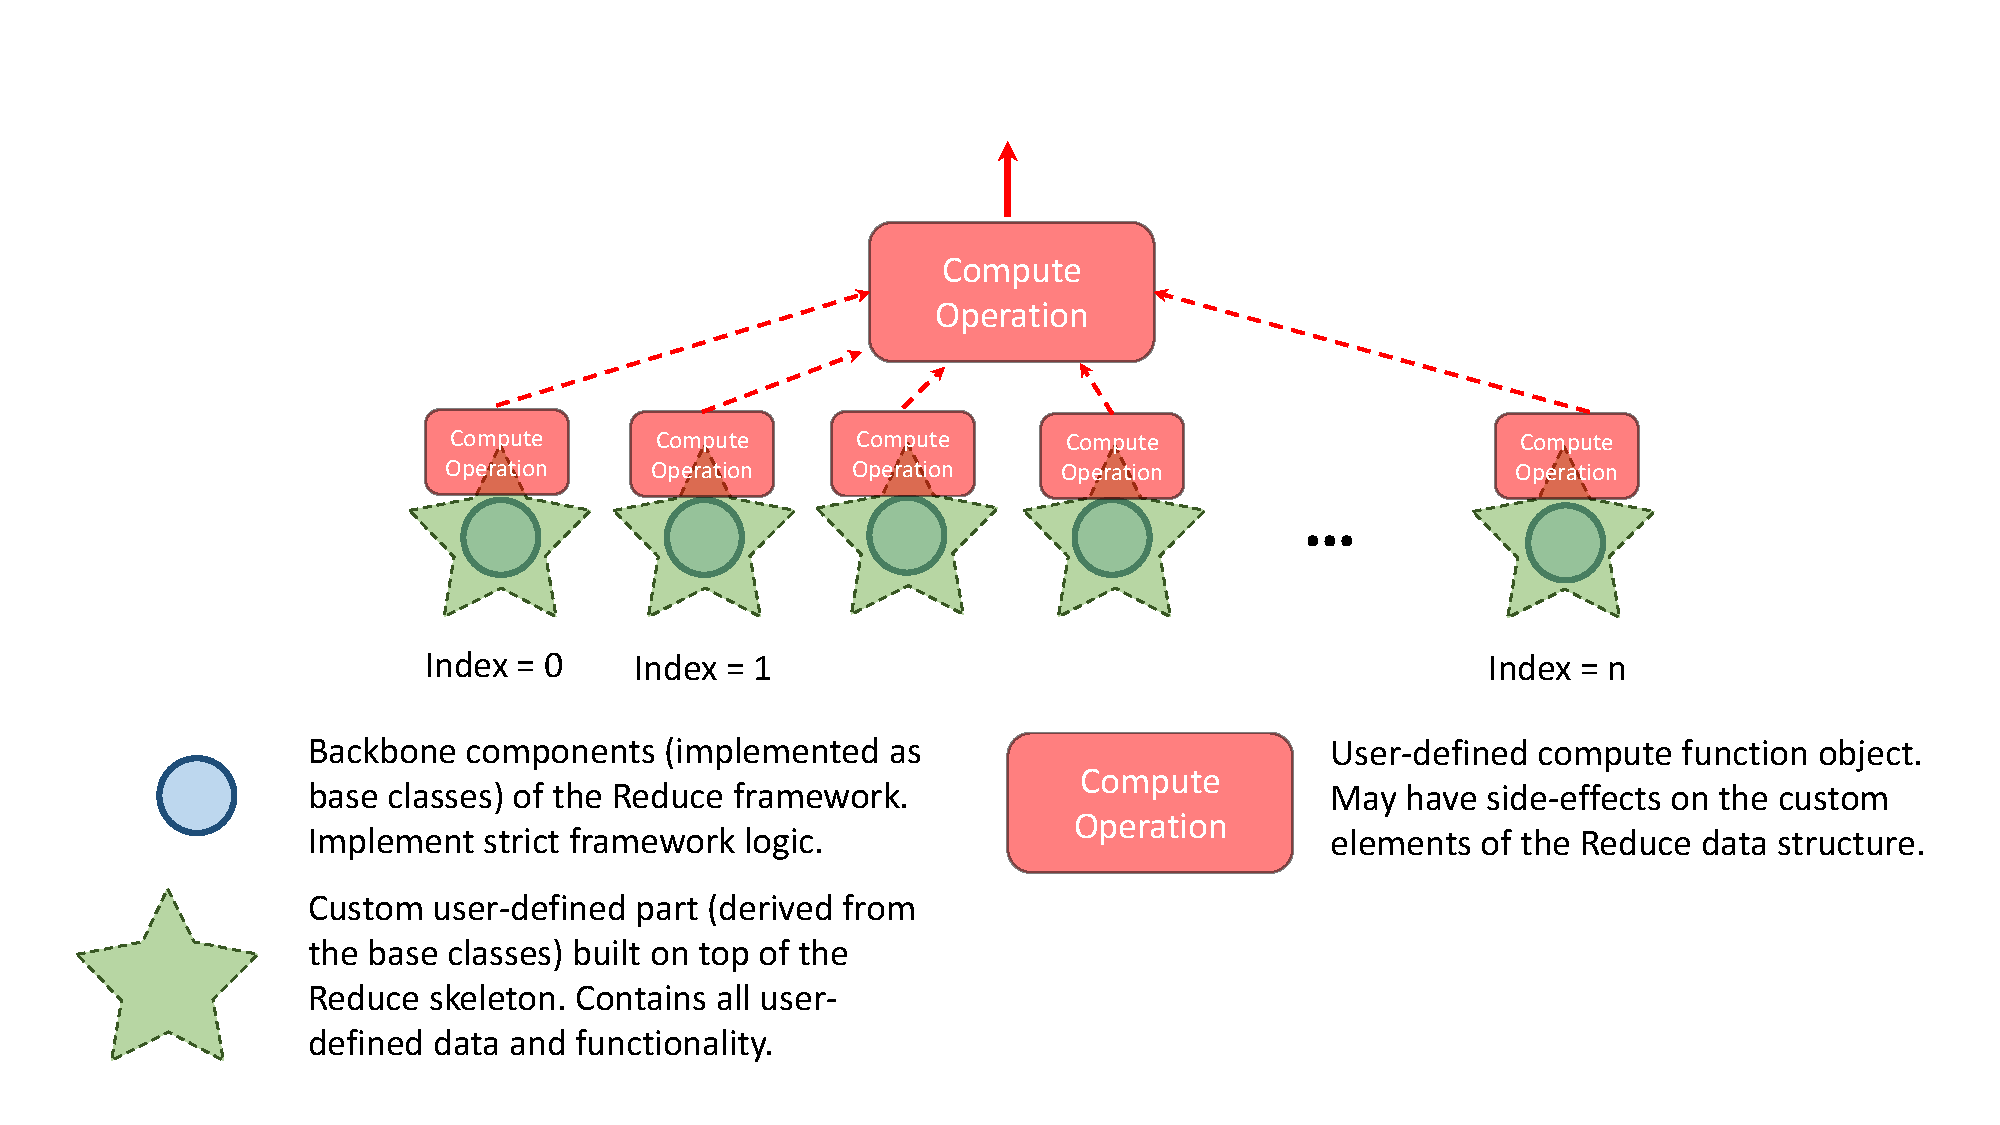
\includegraphics[width=1.0\textwidth]{images/Reduction.pdf}
\caption{An object-oriented design of the Reduce algorithmic skeleton. The design is identical to that of computational frameworks. The two concepts are inter-operable.}
\label{fig:reduce}
\end{figure}
\subsection{Frameworks library design and implementation}
\label{frameworks_library_design}
\quad Despite a number of framework specific differences, all our frameworks stick to the same user interface and design. The design and implementation of computational frameworks library have been done along the curved and iterative path running into numerous dead ends and doing redesign efforts over and over before we managed to get the final library version \cite{frameworks-repo}. The major questions raised during the design process of the library were the trade-off between employing static vs. dynamic polymorphism, interoperability of different frameworks (how do we handle the reduction of folds of folds of reductions like in the case of the \textit{power} benchmark, for instance?), as well as the overall library coherence questions (how to design a common interface for patterns as different as fold and fractal?). But the final design goals have always been clear and follow below.
\begin{description}[style=unboxed,leftmargin=0cm]
\itemsep0em
\item[Modern C++] The implementation of the library is based on the Standard Template Library (STL) data structures, uses move semantics and unique pointers to achieve efficiency and smart memory management. For parallelization library uses OpenMP standard, thus making source code portable. The library is composed of a set of header files with class templates, which are supposed to be included into the user application.
\item[Convenience] We designed the library in an object-oriented fashion with a functional look of its user interfaces and the portability in mind.
\item[Coherence] Despite variations in the prescribed behaviour, all computational frameworks should stick to the same user interface as well as internal design. The coherence would improve inter-operability of different frameworks (say composing a reduction of folds), improve library usability, as well as ease its maintenance and extension. Among less intuitive things, a more general design that handles folds, reductions, fractals, etc. along with all the applications using them altogether will be of the higher quality overall.
\item[Sound design] We strove to use the best software design practices. The user side of the library has been inspired by the LLVM Pass Framework \cite{llvm-compiler-infrastructure} and alike it the library uses the \textit{Curiously Recurring Template Pattern (CRTP)} to decrease the number of template parameters and avoid some of the dynamic polymorphism overheads. The concept of computational frameworks fits exactly into the well-known \textit{algorithm template} pattern and the functional user side is implemented with function objects and higher order template methods following the \textit{command} pattern.
\end{description}
\quad We used 4 Olden benchmarks as an inspiration and guide. Benchmarks \textit{health}, \textit{perimeter} and \textit{treeadd} defined our \textbf{Fractal} computational framework. The \textit{power} benchmark shaped \textbf{Fold} and \textbf{Reduce} frameworks. Moreover, striving for coherence and common interface, the designs of different frameworks had a profound effect on each other.\newline\null
\quad Listing \ref{lst:framework_template_skeleton} shows the essential parts of the final framework design. Initially, custom framework element growth methods such as $Element::grow()$ and $Element::growth\_stop\_condition()$ were specified as separate $Framework<>$ template parameters, but were moved to become virtual functions of the base $Element$ class as a trade-off between static vs. dynamic polymorphism. The template method $Framework<>::compute<ComputeType>()$ is a higher order functional interface, which takes a function object of framework specific type $Framework<>::ComputeFunction<>$ and applies it to the framework along with computing the main result of the $ComputeType$ type. Listing \ref{lst:framework_template_skeleton} shows the one for \textbf{Reduction} class. A user is supposed to override two overloaded operators(), which specify a reduction from a single element complemented with the final combining operation. $Framework<>::grow()$ method defines the backbone data structure and representation of the framework and makes calls to custom user defined functions controlling the growth process.

%\begin{minipage}[t]{\linewidth}
\begin{lstlisting}[caption={Computational framework class template skeleton},label={lst:framework_template_skeleton},language=C++]
template <typename ElemType, typename SeedType>
class Framework {
    public:
        class Element {
            // user-exposed customization iface
            virtual void grow(SeedType) = 0;
            virtual bool growth_stop_condition() { return false; }
        };
        template <typename ComputeType>
        class ComputeFunction {
            public:
            // framework specific application function API
            virtual ComputeType operator()(ElemType& elem) = 0;
            virtual ComputeType operator()(const std::vector<ComputeType>&) = 0;
        };
        void grow(size_t size, SeedType seed) {
            // organise framework elements 
            // into a data structure
            ... = new ElemType(); 
        }
        template<typename ComputeType>
        ComputeType compute(ComputeFunction<ComputeType>& apply_func);
    
    private:
        // framework data structure organisation
        // (list, tree, array, etc.)
};

\end{lstlisting}
%\end{minipage}
\section{Library Deployment}
\label{frameworks_performance}
\subsection{Source Lines Of Code (SLOC) metric  comparison}
\label{frameworks_loc}
\quad Although the Source Lines Of Code (SLOC) metric does not always correctly reflect the program properties (such as comprehensibility, maintainability, etc.), it is still interesting to compare the original legacy implementation of Olden benchmarks against the implementation using our computational frameworks in terms of this metric.\newline\null
\quad Here we need to make some comments. First, the comparison is not completely fair, since the original pointer-based implementation of Olden benchmarks is sequential (only the \textit{power} benchmark contains parallelizing OpenMP pragmas). Whereas our implementation can be made sequential or parallel with just one line of code like \textit{tree.set\_impl\_type(Fractal\_t::ImplType::parallel)} and everything else happens "under the hood". It is also important to note, that we are comparing legacy C vs. C++ implementations. Programs written in C++ tend to be slightly more verbose in terms of SLOC with their class definitions, constructors, destructors, etc. Second, as with any third-party library, before we can use it, we need to perform a setup, which often contains a lot of "boilerplate" code. In the case of computational frameworks the setup implies derivation of custom classes from the base classes of our library, instantiating templates and some other extra syntactical constructions. The business logic of the application can be split into two phases: computational framework \textit{build} and \textit{compute}.\newline\null
\begin{table*}[!ht]{\linewidth}
  \tabulinesep=2pt
  \begin{minipage}{\linewidth}
  \begin{center}
    \begin{tabu}{M{1.4cm}M{1.2cm}M{1.2cm}M{1.2cm}M{1.2cm}M{1.2cm}M{1.2cm}M{1.2cm}M{1.2cm}}
      \hline
      \rowfont{\bfseries}
      \multirow{2}{*}{stage} & \multicolumn{2}{M{2cm}}{power} & \multicolumn{2}{M{2cm}}{health} & \multicolumn{2}{M{2cm}}{perimeter} & \multicolumn{2}{M{2cm}}{treeadd}\\
      & original & abstract & original & abstract & original & abstract & original & abstract\\\hline
      setup & 80 & 170 & 55 & 65 & 15 & 35 & 10 & 30\\
      build & 60 & 50 & 50 & 30 & 50 & 60 & 15 & 1\\
      compute & 380 & 460 & 250 & 230 & 190 & 200 & 60 & 40\\\hline
      \end{tabu}
  \end{center}
  \caption{Implementation SLOC size comparison: original legacy C version (\textit{original}) vs. C++ computational frameworks based one (\textit{abstract}). }
  \label{tab:frameworks_sloc}
  \end{minipage}
\end{table*}%
\quad Table \ref{tab:frameworks_sloc} presents the results. For all 4 benchmarks the setup size is larger in terms of SLOC for the implementation based on our computational frameworks, but after the setup is done we can see some improvement on the \textit{health} benchmark. Parallel C++ version of the benchmark takes less SLOC, than a legacy sequential one. The same is true for \textit{treeadd} benchmark. The \textit{power} benchmark demonstrates the opposite tendency. The computation of the benchmark is composed of the reduction of folds of folds of reductions. Moreover, every fold contains two components: left inject and right fold. These joint points require some additional setting, initialization, and passing of parameters. The latter bloats the code. The \textit{perimeter} benchmark does not show significant differences.
\subsection{Performance study of the library}
\label{frameworks_runtime}
\quad To assess the potential and utility of the concept of computational frameworks, we implemented a prototype library and conducted its thorough performance examination on the subset of Olden benchmarks. We used 4 benchmarks we are interested in. Benchmarks \textit{health}, \textit{treeadd} and \textit{perimeter} fit into our \textbf{Fractal} framework and stress it from different angles. We used the \textit{power} benchmark to test the practical operation of our \textbf{Fold} and \textbf{Reduce} frameworks. We expressed computations in these benchmarks through applicable computational frameworks and have rewritten the original sequential legacy C implementations of the benchmarks with our prototype library in a rejuvenated, structured, well-designed and crucially parallel way. On the opposite side, these benchmarks inspired the concept of computational frameworks and shaped the design of the library. \textit{All our benchmarks have been compiled with GCC 10.1 and -O3 optimization sets. Benchmark running times have been measured with the help of UNIX \textbf{time()} on a powerful compute cluster running Ubuntu 20.04 (focal) and having 64 AMD EPYC 7302 3303 MHz 16-core processors with a total of 0.5 Tb of RAM}.\newline\null
\quad Performance plots below (Figures \ref{fig:performance_health}, \ref{fig:performance_power_reduction_width}, \ref{fig:performance_treeadd}, \ref{fig:performance_perimeter}) show the strengths of the library, as well as its equally important weaknesses. The latter characterize applicability and limitations of the library, rather than the problems of the idea. Although \textit{perimeter} benchmark still demonstrates the potential it also highlights the prototype research nature of the library and shows where it needs an optimization effort. The latter presents a matter of software engineering and not that of a research.\newline\null
\quad The implementation can be easily configured to be sequential or parallel, thus making it easy to conduct measurement experiments. Moreover, the Fractal framework has 2 implementations under the hood. In the most general case the Fractal is based on N-ary unbalanced tree. In this case we allocate it dynamically and every node has an array of pointers to its children. But in the case of a perfect (all leaves are at the same depth and every non-leaf node has all children present) tree, we can allocate all nodes linearly in an array-based heap manner. In the latter case parallelization happens per level, spawning the number of threads equal to the number of nodes at the given depth (provided that enough CPU cores are available). In the general case though we do not know where the growth of the fractal is going to stop and cannot index nodes on the array. Parallelization in the case of unbalanced fractal happens per child: spawning the number of threads equal to the number of children (again, provided that enough CPU cores are available). Figure \ref{fig:balanced_vs_unbalanced} illustrates two implementation strategies and performance plots below compare them. Listing \ref{lst:fractal_parallelization} illustrates "under-the-hood" parallelization of our fractal computational framework in the most general case of unbalanced tree.
\begin{lstlisting}[caption={The "under-the-hood" parallelization of unbalanced Fractal computational framework},label={lst:fractal_parallelization},language=C++]
template <typename ElemType, typename SeedType, int Arity>
template <typename ComputeType>
ComputeType Fractal<ElemType,SeedType,Arity>::Element::compute(ComputeFunction<ComputeType>& compute_func) {
    
    std::vector<ComputeType> ret_vals;
    
    if (!children.empty() && 
        (this->info.level-1 > 0) )
    { 
        if (info.depth < 2) {
            ComputeType tmp[Arity];
            int threads_count = Arity;
            #pragma omp parallel num_threads(threads_count) shared(tmp)
            {
                #pragma omp for schedule(static)
                for (int i = 0; i < Arity; i++) {
                    tmp[i] = children[i]->template compute<ComputeType>(compute_func);
                }
            }

            for (int i = 0; i < Arity; i++) {
                ret_vals.push_back(tmp[i]);
            }
        } else {
            for (int i = 0; i < Arity; i++) {
                ret_vals.push_back(children[i]->template compute<ComputeType>(compute_func));
            }
        }
    }
   
    return compute_func(*(static_cast<ElemType*>(this)), ret_vals);
}
\end{lstlisting}
\begin{figure}[!htb]
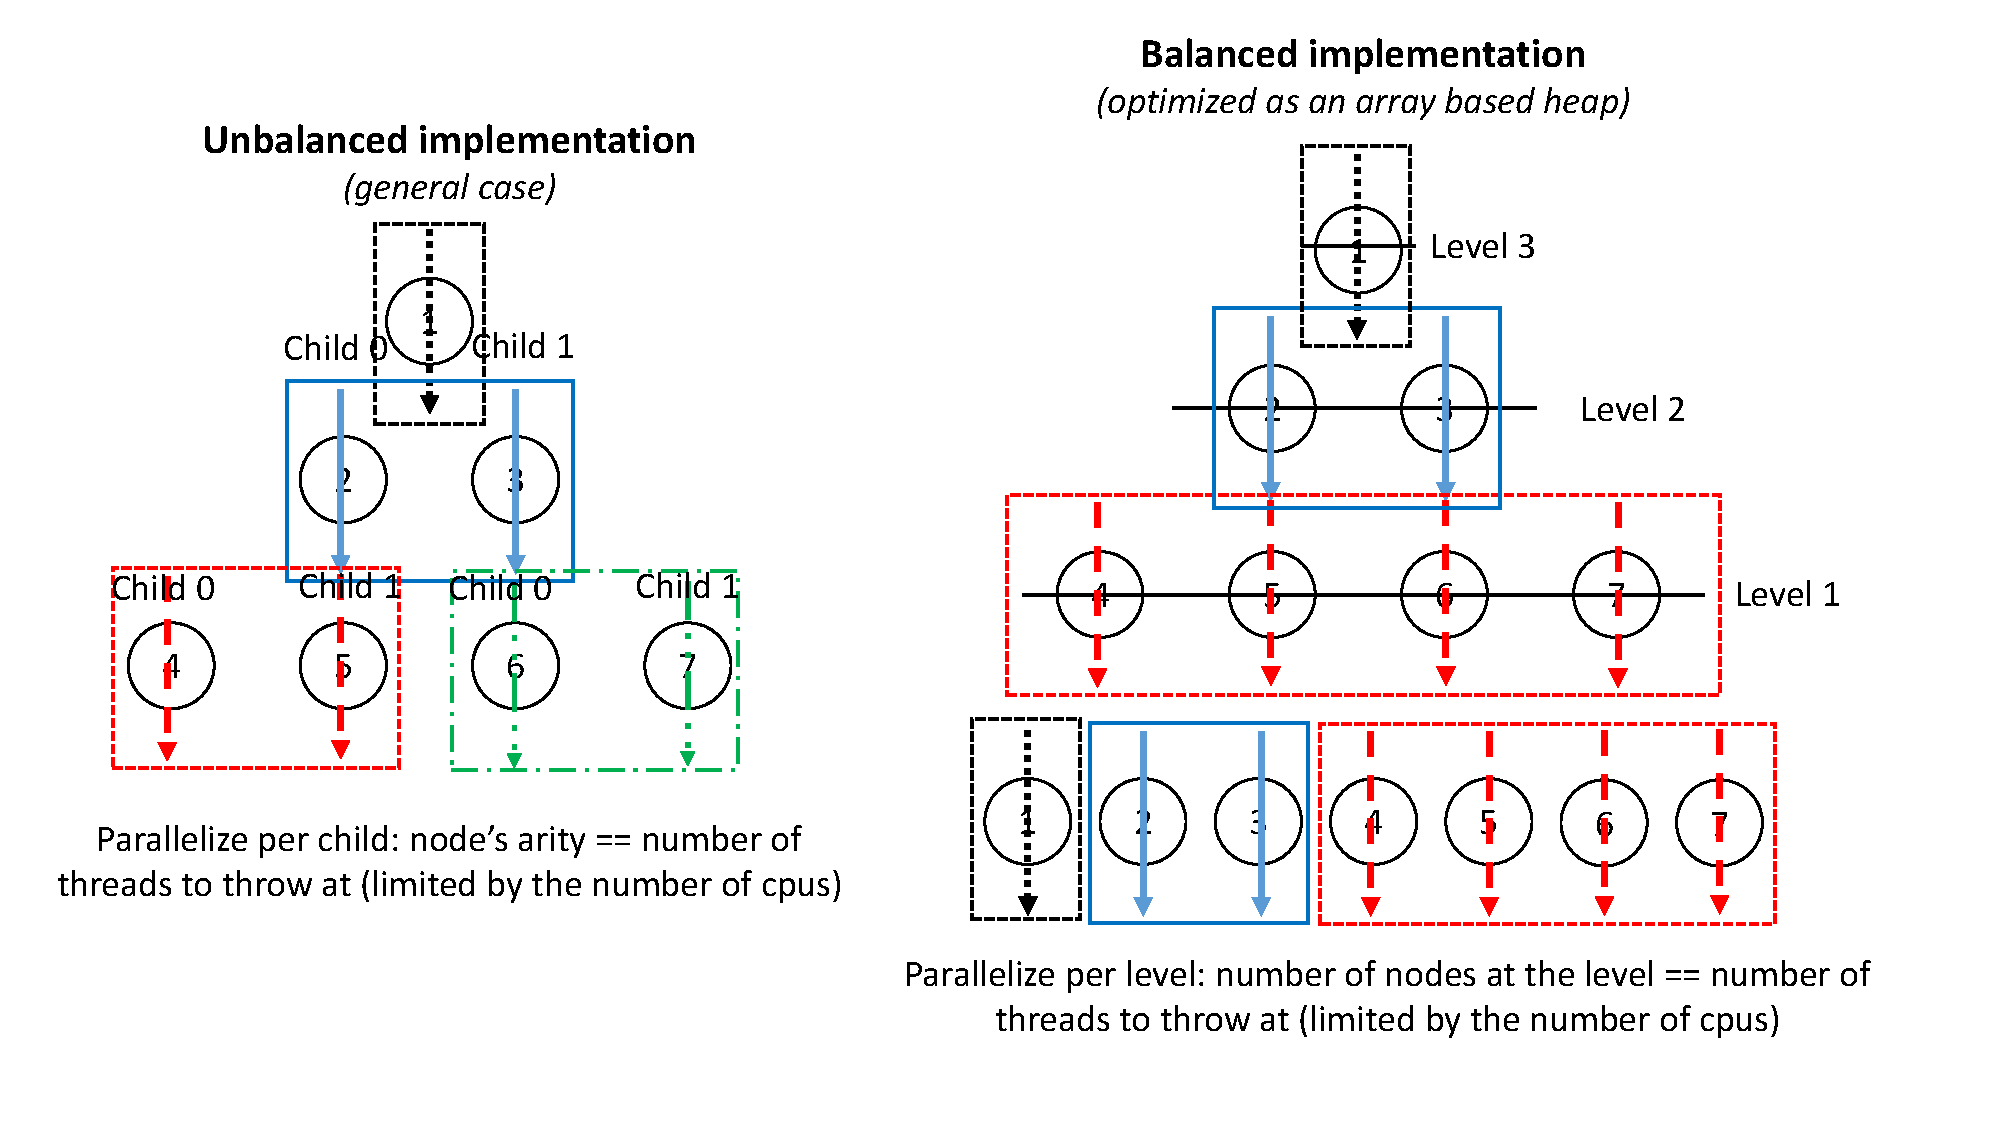
\includegraphics[width=1.0\textwidth]{images/balanced_vs_unbalanced.pdf}
\caption{\textit{Balanced} vs. \textit{Unbalanced} implementations of the fractal framework. Unbalanced implementation handles arbitrary trees and thus is based on pointers. Balanced implementation optimizes the case of a perfect tree and can be implemented with an array.}
\label{fig:balanced_vs_unbalanced}
\end{figure}\newline\null
\quad Figure \ref{fig:performance_health} demonstrates performance of various versions of the \textit{health} benchmark. The benchmark was described in Section \ref{background_benchmarks_olden}. The benchmark grows a tree of hospitals and performs a simulation of the Columbian healthcare system step by step. The number of simulation steps done is plotted on the horizontal axis. The time a simulation took is plotted on a vertical axis. Nodes of the tree, which represent hospitals grow various lists of patients. As simulation goes the lists grow and the nodes become heavier. In other words, the state of the benchmark becomes bigger. The latter has an accumulating effect and contributes to the workload. We can see this phenomenon reflected in an exponential time growth of the sequential version. Parallel versions diminish this time by tackling the task with several threads. This results into 5-6x speedups of the parallel versions relative to sequential ones. This benchmark is an ideal one to tackle with our fractal framework. And indeed, as Figure \ref{fig:performance_health} shows, the thick lines representing the real time (wall clock time) indicate that a parallel versions consistently outperform sequential versions. The sequential versions of our library perform roughly as well as the original legacy C implementation (thin lines vs. a thick \textit{original} line). The latter shows that our library does not introduce any overheads on a benchmark with a significant workload. Dotted lines show the CPU time and illustrate how much of the CPU time has been used by several computational threads of the application. This measure can be used to judge on the aggressiveness of parallelization. 
\begin{figure}[!htb]
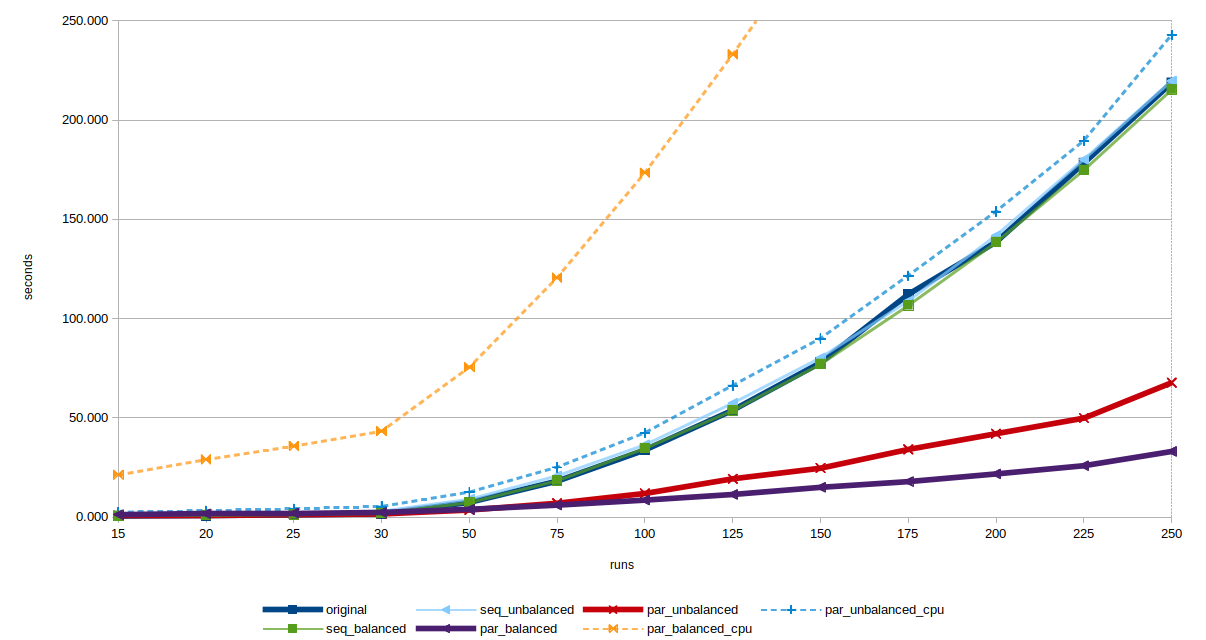
\includegraphics[width=1.0\textwidth]{images/health_depth_10.png}
\caption{Library performance on the \textit{health} benchmark. The legacy C implementation is represented by a thick \textit{original} line. Implementations of the benchmark based on our library are represented by 2 thick (\textit{parallel balanced} and \textit{unbalanced}) and 2 thin (\textit{sequential balanced} and \textit{unbalanced}) lines. Dotted lines represent the CPU time, which is not the real time and has a secondary importance. CPU time reflects the computational workload as we throw several threads at a task and can be used to judge on parallelization aggressiveness.}
\label{fig:performance_health}
\end{figure}\newline\null
\quad Figure \ref{fig:performance_power_reduction_width} illustrates the results for the \textit{power} benchmark. The benchmark performs a workload of scientific computations. The pattern is basically a reduction of folds of folds of reductions. So, the benchmark tests our \textbf{Fold} and \textbf{Reduce} frameworks. We can vary the width of reductions as well as the depth of folds to get various amounts of workload. The benchmark runs repeatedly until the computation result falls withing the set epsilon error. Figure \ref{fig:performance_power_reduction_width} illustrates how the running time of the benchmark scales with an increasing top level reduction width. The latter increases the workload and one can see the growing running time of the sequential original legacy C version. The sequential version based on our library runs roughly as well as the original one, while the parallel version consistently outperforms both sequential versions. Dotted line again represents the CPU time and not the real time. CPU time approximately reflects how many threads were used to run the benchmark. As a validation, one can see that CPU time divided by parallel wall clock time roughly corresponds to the reduction width. Behaviour of the \textit{power} benchmark does not change significantly, when we vary reduction widths or fold depths. We do not include the other experiments we ran, as they do not change the picture.
\begin{figure}[!htb]
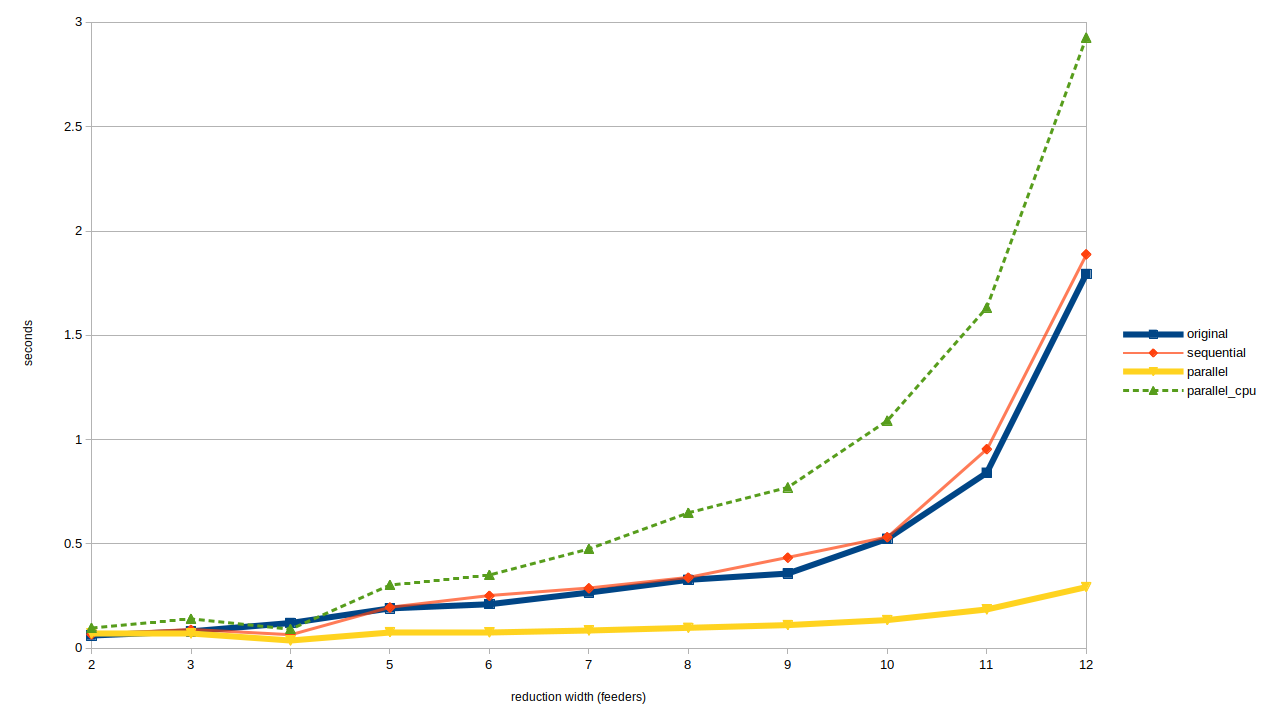
\includegraphics[width=1.0\textwidth]{images/power_reduction_width.png}
\caption{Library performance on the \textit{power} benchmark. We vary the top level (feeders) reduction width to scale the workload.}
\label{fig:performance_power_reduction_width}
\end{figure}\newline\null
\quad The \textit{health} and the \textit{power} benchmarks show the strengths of our library. The \textit{treeadd} and \textit{perimeter} benchmarks highlight its weaknesses. The weaknesses stress the research prototype nature of the library and show places for further optimization effort. Figure \ref{fig:performance_treeadd} shows the behaviour of the \textit{treeadd} benchmark. This benchmark grows a tree with values at its nodes. Then it runs iteratively computing the reduction over the tree and updating node values. The computation is very lighweight. Basically it is just one addition per node processing. The state is minimal and does not accumulate as we run the benchmark over and over. One can see a roughly linear running time of the original legacy C version. Overheads of our sequential library versions are striking for such a small benchmark. Although the asymptotic complexity of all shown versions is the same, various bookkeeping overheads of the library diminish performance relative to the original version with just a single addition per node as the workload. These overheads can be optimized away with some engineering effort, but present in the research prototype library. The more threads we throw the bigger our overheads become. One can see it looking at the running time of balanced and unbalanced versions. It is worthless to tackle such a small benchmark with our library.      
\begin{figure}[!htb]
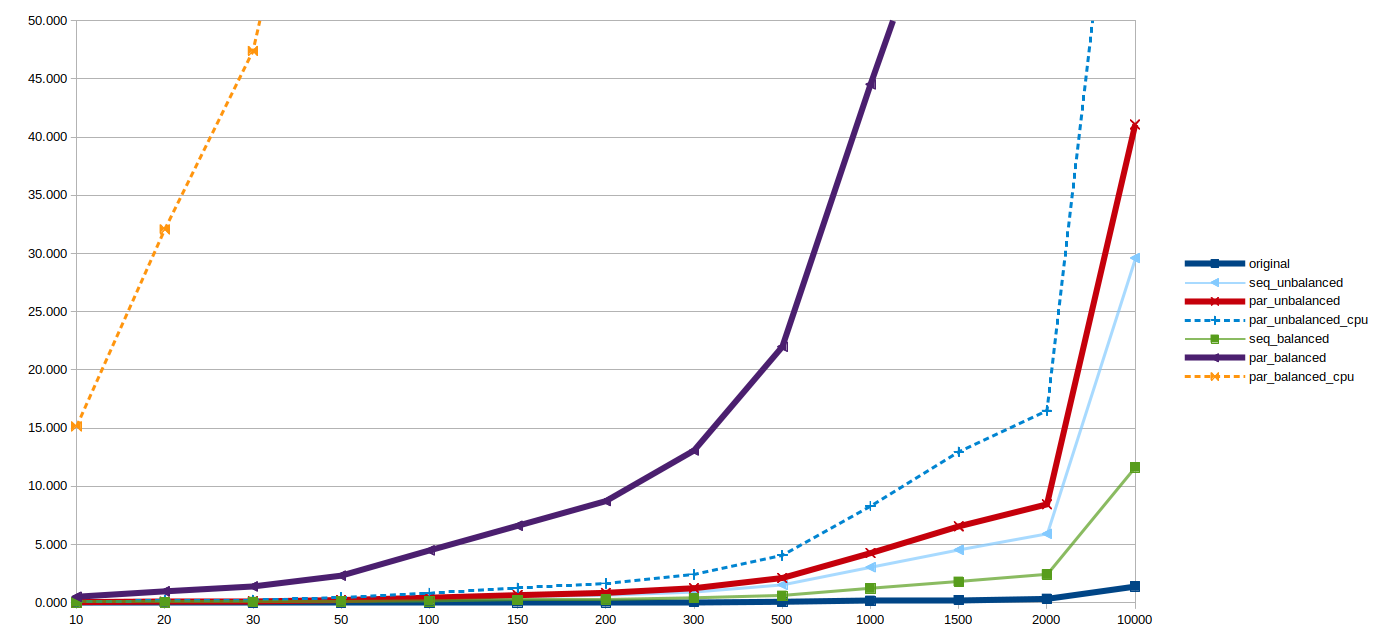
\includegraphics[width=1.0\textwidth]{images/treeadd_depth_16.png}
\caption{Library performance on the \textit{treeadd} benchmark.}
\label{fig:performance_treeadd}
\end{figure}\newline\null
\quad The \textit{perimeter} benchmark shows a different picture, but still highlights the current weaknesses of the library implementation. Figure \ref{fig:performance_perimeter} shows the bar chart. The benchmark does not run an iterative simulation as the 3 other benchmarks do - it is a single perimeter computation. Horizontal axis plots the depth of the tree underlying perimeter computation, a workload size in other words. As usual, the vertical axis plots the time it took to run the computation. As the benchmark is based on an unbalanced tree version we cannot run it with a balanced implementation. Here we have only the original sequential legacy C implementation, the sequential implementation based on our library and its parallel counterpart. One can see that the benchmark also highlights the current implementation problems: original does better than sequential. At the same time the benchmark has a potential: there is a good parallel speedup when we compare the sequential versus parallel library based versions.
\begin{figure}[!htb]
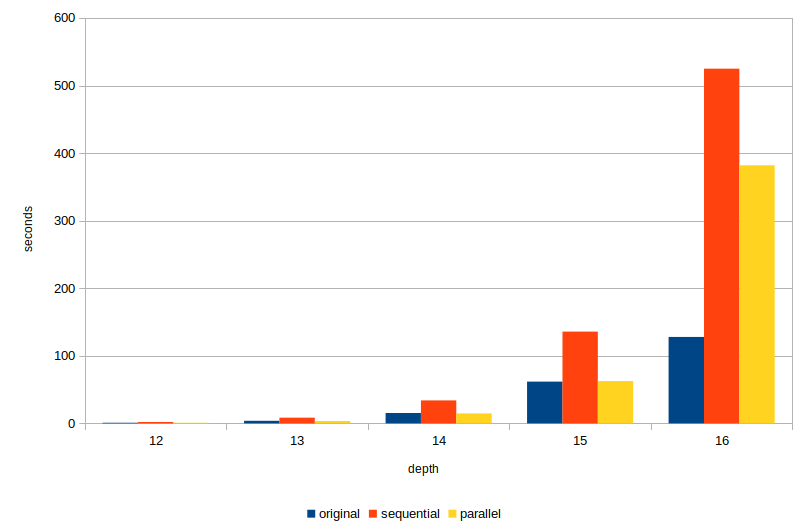
\includegraphics[width=1.0\textwidth]{images/perimeter.png}
\caption{Library performance on the \textit{perimeter} benchmark. Horizontal axis plots the depth of the perimeter tree (see Section \ref{background_benchmarks_olden}). Vertical axis shows the time it takes to compute a single perimeter value with various tree depths (splitting granularity).}
\label{fig:performance_perimeter}
\end{figure}

\section{Limitations & Future work}
\label{frameworks_future_work}
\subsection{Limitations}
\label{frameworks_limitations}
\quad The limitations of our computational frameworks largely come as the implications of unconstrained side effects. Compared to pure functional patterns our computational frameworks give a programmer more freedom by allowing to leave side effects, but this comes at the price of programmers having more responsibility. It is an interesting trade-off by itself, but a programmer still needs to understand computational patterns our frameworks support and a high level parallelization they do to prevent possible race conditions. Aside conforming to a certain interface, our computational frameworks do not impose any particular restrictions on operator functions and provide a programmer with a freedom. Obviously, our computational frameworks are not universal and are limited to only those problems they are applicable to.
\subsection{Future work}
\label{frameworks_fw}
\quad The Chapter \ref{related_work} presents an overview of related work on various automatic and semi-automatic software parallelization methods. Automatically parallelizing compilers are restricted by the limitations of static program analysis. As a workaround solution, various researchers have proposed techniques on automatic data structure and algorithmic skeleton recognition. The application of these techniques for the real world code could be exacerbated by the problem of algorithm and data structure inseparability.\newline\null
\quad The concept of computational frameworks and the prototype library could lay a foundation towards an alternative automatic parallelization technique. We believe that it is possible to automatically recognise computational frameworks in the suite of Olden benchmarks. Alike the work \cite{skeletons-static}, the recognition technique could be based on the static analysis of program's AST. Figure \ref{fig:parallelization_scheme} shows the scheme. It takes an original legacy C source code, where we supposedly have a computation that fits into one or several of our frameworks. The task of the recognizer is to identify a computational pattern. Like in the case of the \textit{health} Olden benchmark we have a recursive \textit{grow()} and \textit{compute()} procedures, which build and process the tree correspondingly. That recursive pattern can be matched to a fractal framework. The next step would be to strip the code corresponding and implementing the pattern (\textit{backbone logic}) and leave the rest as the \textit{business logic}. The business logic must be further classified into various computational framework template class methods (like \textit{grow()}, \textit{growth\_stop\_condition()}, \textit{inject()}, etc.). Then, the class template must be instantiated with the business logic inserted into the right places. Once that is done, the parallelization is done, as the compiler will take care of everything else.
\begin{figure}[!htb]
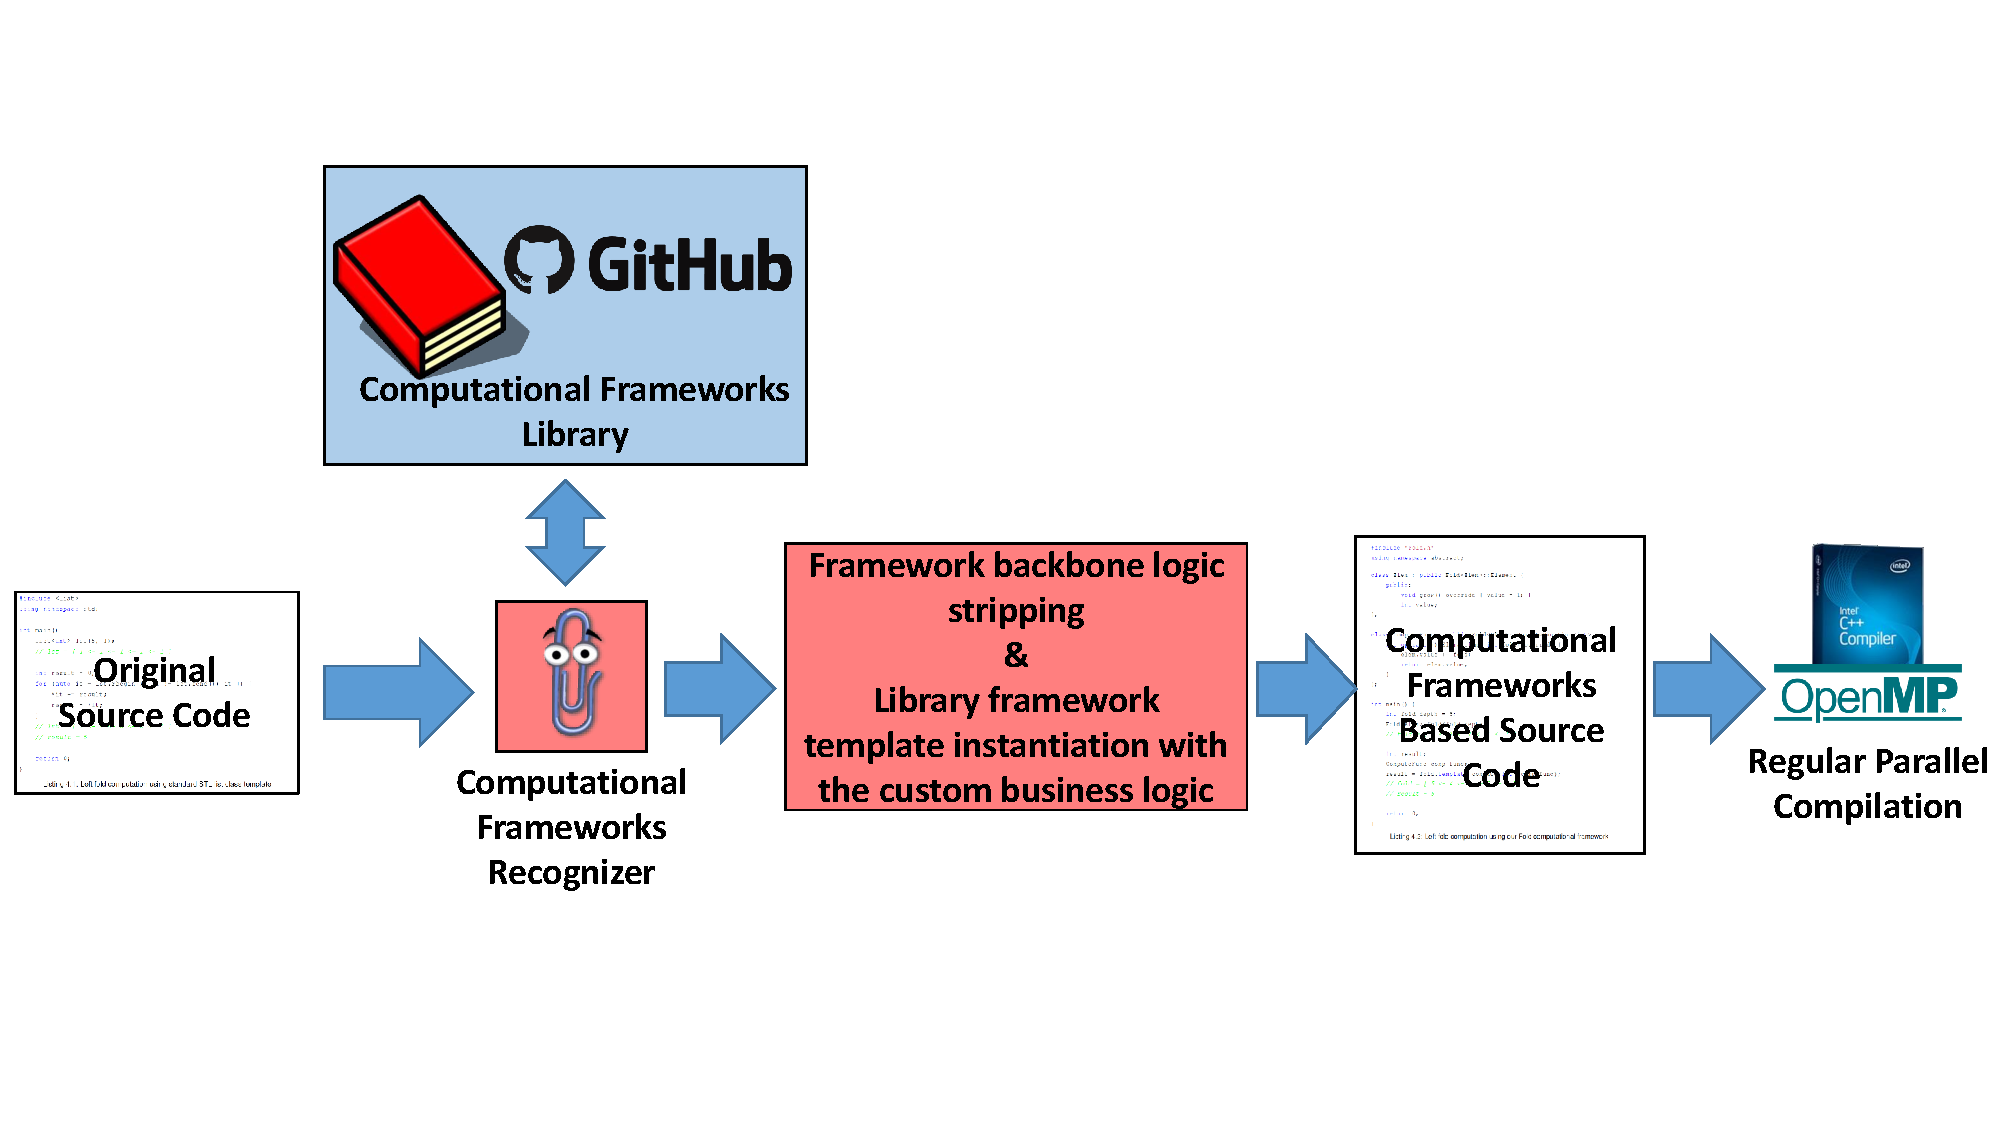
\includegraphics[width=1.0\textwidth]{images/parallelization_scheme.pdf}
\caption{An alternative software parallelization scheme based on our library of computational frameworks.}
\label{fig:parallelization_scheme}
\end{figure}\newline\null
\quad Technically, for benchmarks as simple as Olden the technique can work on the level of compiler's front end: source code or an abstract syntax tree (AST). That sets the technique apart from the regular parallelization approaches based on dependence graphs and working on the level of compiler's intermediate representation (IR).

%%